% -*- root: Dissertation.tex -*-
\documentclass[Dissertation.tex]{subfiles}
\begin{document}
\graphicspath{{../Figures/}}
\chapter{Space-Time DPG for Compressible Navier-Stokes}
\label{sec:compressible}
\section{Motivation}

The compressible Navier-Stokes equations are
\begin{align}
\frac{\partial}{\partial t}\svectthree{\rho}{\rho\bfu}{\rho e_0}
+\Div\svectthree{\rho\bfu}{\rho\bfu\otimes\bfu+p\bbI-\mathbb{T}}{\rho\bfu e_0+\bfu p+\bfq-\bfu\cdot\mathbb{T}}
%TODO: Possible error above. cfd-online seems to have T^T
=\svectthree{f_c}{\bff_m}{f_e}\,,
\end{align}
where $\rho$ is the density, $\bfu$ is the velocity, $p$ is the pressure, $\bbI$ is the identity matrix,
$\mathbb{T}$ is the deviatoric stress tensor or viscous stress, $e_0$ is the total energy, $\bfq$ is the heat flux, 
and $f_c$, $\bff_m$, and $f_e$ are the source terms for the continuity, momentum, and energy equations, respectively.
Assuming Stokes hypothesis that $\lambda=-\frac{2}{3}\mu$, 
\begin{equation*}
	\mathbb{T}=2\mu\bfS^*=2\mu\LRs{\frac{1}{2}\LRp{\Grad\bfu+\LRp{\Grad\bfu}^T}-\frac{1}{3}\Div\bfu\bbI}\,,
\end{equation*}
where $\bfS^*$ is the trace-less viscous strain rate tensor.
In order to work with standard finite element spaces, we introduce $\bbD=\mu\Grad\bfu$, so that 
$\mathbb{T}=\LRp{\bbD+\bbD^T-\frac{2}{3}\trace(\bbD)\bbI}$.
The heat flux is given by Fourier's law:
\begin{equation*}
	\bfq=-C_p\frac{\mu}{Pr}\Grad T\,,
\end{equation*}
where $C_p$ is the specific heat at constant pressure and $Pr$ is the laminar Prandtl number: $Pr:=\frac{C_p\mu}{\lambda}$.
We need to close these equations with an equation of state. An ideal gas assumption gives
\begin{equation*}
	\gamma:=\frac{C_p}{C_v}\,,\quad p=\rho RT\,,\quad e=C_v T\,,\quad C_p-C_v=R\,,
\end{equation*}
where $\gamma$ is the ratio of specific heats, $C_v$ is the specific heat at constant volume, $R$ is the gas constant,
$e$ is the internal energy, $T$ is the temperature,
and $\gamma$, $C_p$, $C_v$, and $R$ are constant properties of the fluid.
The total energy is defined by
\begin{equation*}
	e_0=e+\frac{1}{2}\bfu\cdot\bfu\,.
\end{equation*}

We can write our first order system of equations in space-time as follows:
\begin{subequations}
\label{eq:compressibleNSFirstOrder}
\begin{align}
	\frac{1}{\mu}\bbD-\Grad\bfu&=0\\
	\frac{Pr}{C_p\mu}\bfq+\Grad T&=0\\
	\Divxt\vecttwo{\rho\bfu}{\rho}&=f_c\\
	\Divxt\vecttwo{\rho\bfu\otimes\bfu+\rho RT\bbI-\LRp{\bbD+\bbD^T-\frac{2}{3}\trace(\bbD)\bbI}}
	{\rho\bfu}&=\bff_m\\
	\Divxt\vecttwo{\rho\bfu\LRp{C_v T+\frac{1}{2}\bfu\cdot\bfu}+\bfu\rho RT+\bfq
	-\bfu\cdot\LRp{\bbD+\bbD^T-\frac{2}{3}\trace(\bbD)\bbI}}
	{\rho\LRp{C_v T+\frac{1}{2}\bfu\cdot\bfu}}&=f_e\,,
\end{align}
\end{subequations}
where our solution variables are $\rho$, $\bfu$, $T$, $\bbD$, and $\bfq$.

We can simplify the following discussion by introducint the following notation. 
The conserved quantities for each equation are:
\begin{align*}
C_c&:=\rho\\
\bfC_m&:=\rho\bfu\\
C_e&:=\rho(C_v T+\frac{1}{2}\bfu\cdot\bfu)\,.
\end{align*}
while the Euler fluxes are:
\begin{align*}
\bfF_c&:=\rho\bfu\\
\mathbb{F}_m&:=\rho\bfu\otimes\bfu+\rho RT\bbI\\
\bfF_e&:=\rho\bfu\LRp{C_v T+\frac{1}{2}\bfu\cdot\bfu}+\bfu\rho RT\,,
\end{align*}
and the viscous fluxes are:
\begin{align*}
\bfK_c&:=\boldsymbol 0\\
\bbK_m&:=\LRp{\bbD+\bbD^T-\frac{2}{3}\trace(\bbD)\bbI}\\
\bfK_e&:=-\bfq+\bfu\cdot\LRp{\bbD+\bbD^T-\frac{2}{3}\trace(\bbD)\bbI}\,.
\end{align*}
The constitutive terms are:
\begin{align*}
\bbM_{\bbD}&:=\bbD\\
\bfM_{\bfq}&:=\frac{Pr}{C_p}\bfq\,
\end{align*}
and the constitutive relations are:
\begin{align*}
\bfG_{\bbD}&:=\bfu\\
G_{\bfq}&:=-T\,.
\end{align*}

Multiplying \eqref{eq:compressibleNSFirstOrder} by test functions $\bbS\in\bbH(\text{div},Q)$,
$\bftau\in\HdivxQ$, $v_c\in\HonextQ$, $\bfv_m\in\mathbf{H}_{xt}^1(Q)$, $v_e\in\HonextQ$ and integrating by parts,
we get
\begin{subequations}
\label{eq:compressibleNSNonlinear}
\begin{align}
	\LRp{\frac{1}{\mu}\bbM_\bbD,\bbS}+\LRp{\bfG_\bbD,\Div\bbS}-\LRa{\hat\bfu,\bbS\bfn_x}&=0\\
	\LRp{\frac{1}{\mu}\bfM_{\bfq},\bftau}+\LRp{G_{\bfq},\Div\bftau}+\LRa{\hat T,\tau_n}&=0\\
	-\LRp{\vecttwo{\bfF_c-\bbK_c}{C_c},\Gradxt v_c}+\LRa{\hat t_c,v_c}&=\LRp{f_c,v_c}\\
	-\LRp{\vecttwo{\bbF_m-\bbK_m}{\bfC_m},\Gradxt\bfv_m}+\LRa{\hat\bft_m,\bfv_m}&=\LRp{\bff_m,\bfv_m}\\
	-\LRp{\vecttwo{\bfF_e-\bfK_e}{C_e},\Gradxt v_e}+\LRa{\hat t_e,v_e}&=\LRp{f_e,v_e}\,,
\end{align}
\end{subequations}
where 
\begin{equation*}
\begin{aligned}
\hat\bfu&=\trace(\bfu)\\
\hat T&=\trace(T)\\
\hat t_c&=\trace\LRp{\bfF_c-\bfK_c}\cdot\bfn_x+\trace\LRp{C_c}n_t\\
\hat\bft_m&=\trace\LRp{\bbF_m-\bbK_m}\cdot\bfn_x+\trace\LRp{\bfC_m} n_t\\
\hat t_e&=\trace\LRp{\bfF_e-\bfK_e}\cdot\bfn_x+\trace\LRp{C_e}n_t\,.
\end{aligned}
\end{equation*}
We can further simplify this by introducing group terms and group variables:
\begin{align*}
C&:=\LRc{C_c\,,\, \bfC_m\,,\, C_e}\\
F&:=\LRc{\bfF_c\,,\, \bbF_m\,,\, \bfF_e}\\
K&:=\LRc{\bfK_c\,,\, \bbK_m\,,\, \bfK_e}\\
M&:=\LRc{\bbM_{\bbD}\,,\, \bfM_{\bfq}}\\
G&:=\LRc{\bfG_{\bbD}\,,\, G_{\bfq}}\\
f&:=\LRc{f_c\,,\, \bff_m\,,\, f_e}\\
W&:=\LRc{\rho\,,\,\bfu\,,\,T}\\
\hat W&:=\LRc{\hat\bfu\,,\,-\hat T}\\
\Sigma&:=\LRc{\bbD,\bfq}\\
\hat t&:=\LRc{\hat t_e\,,\,\hat\bft_m,\,,\,\hat t_e}\\
\Psi&:=\LRc{\bbS\,,\,\bftau}\\
V&:=\LRc{v_c\,,\,\bfv_m,\,,\,v_e}\,.
\end{align*}
Our final nonlinear variational formulation looks very similar to what we had for convection-diffusion:
\begin{align*}
\LRp{\frac{1}{\mu}M,\Psi}+\LRp{G,\Div\Psi}-\LRa{\hat W,\Psi\cdot\bfn_x}&=0\\
-\LRp{\vecttwo{F-K}{C},\Gradxt V}+\LRa{\hat t,V}&=\LRp{f,V}\,.
\end{align*}

With appropriate change of varialbes, we could use this same form to consider a solution in terms
of either conservation variables or entropy variables, 
a topic we briefly consider in Appendix \ref{sec:VariableComparison}.


\section{Linearization}
We again begin by splitting our residual into trace and volume terms:
\[
R(W,\hat W,\hat t) = R(W) + R(\hat W,\hat t)\,,
\]
where
\[
R(W)=
\LRp{\frac{1}{\mu}M,\Psi}+\LRp{G,\Div\Psi}
-\LRp{\vecttwo{F-K}{C},\Gradxt V}-\LRp{f,V}\,,
\]
and
\[
R(\hat W,\hat t)=
-\LRa{\hat W,\Psi\cdot\bfn_x}
+\LRa{\hat t,V}\,.
\]
And again $R(\hat W,\hat t)$ is already linear, so we only need to linearize terms dependent on $W$.
Let $W=\tilde W+\Delta W$, where $\tilde W$ is the previous solution in a Newton iteration and 
$\Delta W$ is the update. We linearize about $\tilde W$ so that our linear problem becomes
\[
\pd{R(\tilde W)}{W}\Delta W+R(\hat W,\hat t)=-R(\tilde W)\,,
\]
with unknowns $\Delta W$, $\hat W$, and $\hat t$.
The full definitions for these linearized terms can be found in Appendix \ref{sec:VariableComparison}.

\section{Robust Test Norms}
The adjoint equations are:
\begin{align*}
\frac{1}{\mu}M^*(\Psi)+K^*(\Grad V)&=\vecttwo{\frac{1}{\mu}\bbM_{\bbD}^*(\bbS)}{\frac{1}{\mu}\bfM_{\bfq}^*(\bftau)}
+\vecttwo{\bbK_{\bbD}^*(\Grad V)}{\bfK_{\bfq}^*(\Grad V)}\\
-\vecttwo{F^*}{C^*}(\Gradxt V)+G^*(\Grad\Psi)&=-\vectthree
{F_c^*(\Grad V)+C_c^*(V_{,t})}
{\bfF_m^*(\Grad V)+\bfC_m^*(V_{,t})}
{F_e^*(\Grad V)+C_e^*(V_{,t})}
+\vectthree
{G_c^*(\Grad\Psi)}
{\bfG_m^*(\Grad\Psi)}
{G_e^*(\Grad\Psi)}\,,
\end{align*}
where
these terms can be developed by analyzing the bilinear form and grouping terms according to trial variable:
\begin{align*}
M_\bbD^*\bbS&=\bbS\\
M_{\bfq}^*\bftau&=\frac{Pr}{C_p}\bftau\\
K_\bbD^*\Grad V&=\Grad\bfv_m+(\Grad\bfv_m)^T-\frac{2}{3}\Div\bfv_m\bbI
\\&\quad
+\tilde\bfu\otimes\Grad v_e+(\tilde\bfu\otimes\Grad v_e)^T-\frac{2}{3}\tilde\bfu\cdot\Grad v_e\bbI\\
K_{\bfq}^*\Grad V&=-\Grad v_e\\
\bfF_c^*\cdot\Grad V&=
\tilde\bfu\cdot\Grad v_c
+\tilde\bfu\otimes\tilde\bfu:\Grad\bfv_m+R\tilde T\Div\bfv_m
+C_v\tilde T\tilde\bfu\cdot\Grad v_e
\\&\quad
+\frac{1}{2}\tilde\bfu\cdot\tilde\bfu\tilde\bfu\cdot\Grad v_e+R\tilde T\tilde\bfu\cdot\Grad v_e\\
%
\bfC_c^*\cdot V_{,t}&=v_{c,t}+\tilde\bfu\cdot\bfv_{m,t}+(C_v\tilde T+\frac{1}{2}\tilde\bfu\cdot\tilde\bfu)v_{e,t}\\
%
\bfF_m\cdot\Grad\bfv_m&=\tilde\rho\Grad v_c
+(\Grad\bfv_m+(\Grad\bfv_m)^T)\tilde\rho\tilde\bfu
+C_v\tilde T\tilde\rho\Grad v_e
\\&\quad
+\frac{1}{2}\tilde\rho\tilde\bfu\cdot\tilde\bfu\Grad v_e+\tilde\rho\tilde\bfu\tilde\bfu\cdot\Grad v_e
+R\tilde T\tilde\rho\Grad v_e\\ 
&\quad-\tilde{\bbD}\Grad v_e-(\tilde{\bbD})^T\Grad v_e+\frac{2}{3}\trace(\tilde{\bbD})\Grad v_e
\\
%
\bfC_m^*\cdot V_{,t}&=\tilde\rho\bfv_{m,t}+\tilde\rho\tilde\bfu v_{e,t}\\
%
\bfF_e^*\cdot\Grad V&=R\tilde\rho\Div\bfv_m+C_v\tilde\rho\tilde\bfu\cdot\Grad v_e+R\tilde\rho\tilde\bfu\cdot\Grad v_e\\
%
\bfC_e^*\cdot V_{,t}&=C_v\tilde\rho v_{e,t}\\
%
\bfG_c^*\Grad\Psi&=0\\
%
\bfG_m^*\Grad\Psi&=\Div\bbS\\
%
\bfG_e^*\Grad\Psi&=-\Div\bftau
\,.
\end{align*}
% where the various terms are defined in Appendix \ref{sec:VariableComparison}.
We develop analogous robust norm:
\begin{align*}
\norm{\LRp{V,\Psi}}_{V,K}^2 &\coloneqq
\norm{F^*+C^*}_K^2
+ \mu\norm{K^*}_K^2
+ \min\LRp{\frac{\mu}{h^2},1}\norm{V}^2_K
\\\nonumber&\quad
+ \norm{G^*}_K^2
+ \min\LRp{\frac{1}{\mu},\frac{1}{h^2}}\norm{M^*}_K^2\,,
\end{align*}
coupled robust norm
\begin{align*}
\norm{\LRp{V,\Psi}}_{V,K}^2 &\coloneqq
\norm{F^*+C^*}_K^2
+ \mu\norm{K^*}_K^2
+ \min\LRp{\frac{\mu}{h^2},1}\norm{V}^2_K
\\\nonumber&\quad
+ \norm{G^*-F^*-C^*}_K^2
+ \min\LRp{\frac{1}{\mu},\frac{1}{h^2}}\norm{M^*}_K^2\,,
\end{align*}
and NSDecoupled norm:
\begin{align*}
\norm{\LRp{V,\Psi}}_{V,K}^2 &\coloneqq
\norm{F^*+C^*}_K^2
+ \norm{K^*}_K^2
+ \norm{V}^2_K
\\\nonumber&\quad
+ \norm{G^*}_K^2
+ \frac{1}{h^2}\norm{M^*}_K^2\,.
\end{align*}


\section{Numerical Experiments}
% \subsection{1D Space-Time Problems}
\subsection{Sod Shock Tube}
% Re=1e4, p=2, delta_p=2, nlMaxIters=10, rampRe, coarseRe=1e2

\begin{figure}[ht]
\centering
\begin{subfigure}[t]{0.45\textwidth}
\centering
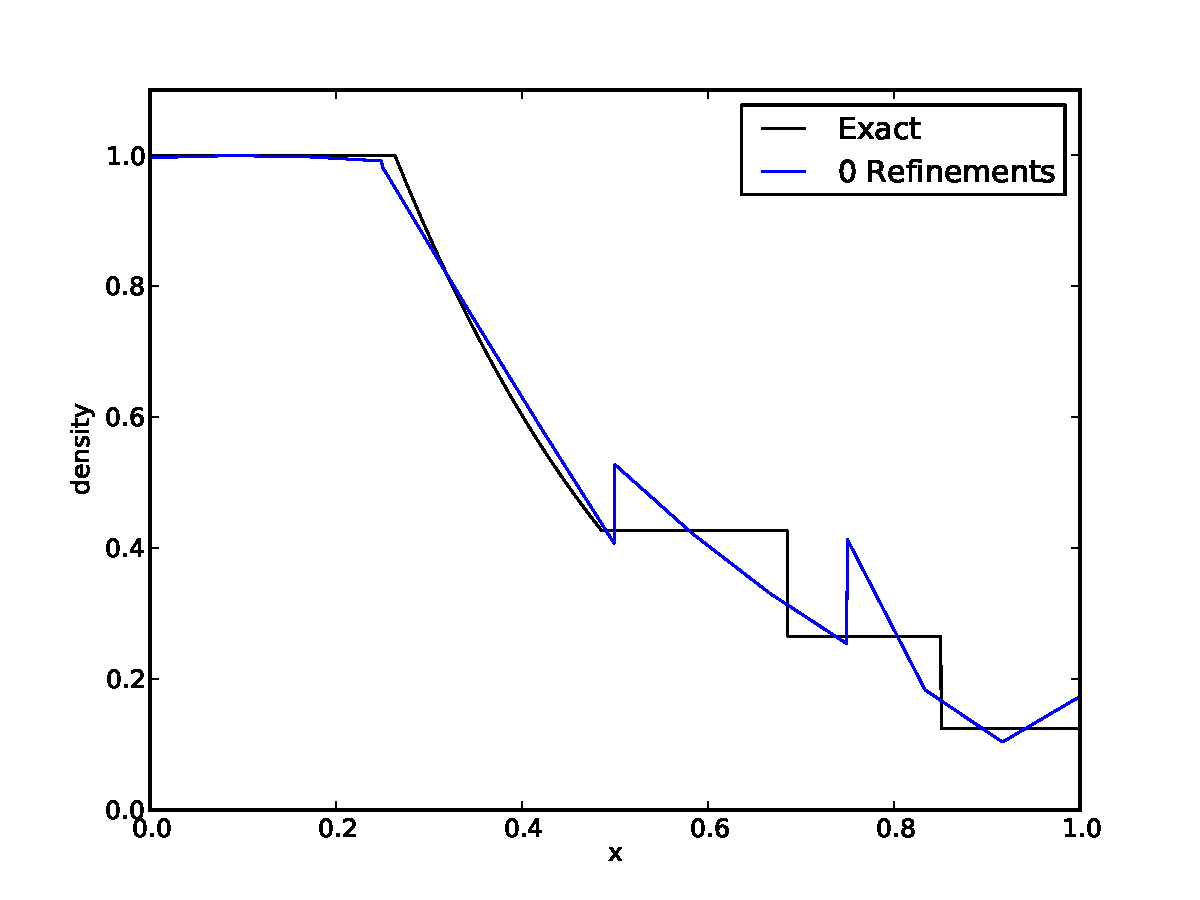
\includegraphics[width=\textwidth]{Dissertation/Sod/Robust-den1.pdf}
\caption{Density}
\end{subfigure}
\begin{subfigure}[t]{0.45\textwidth}
\centering
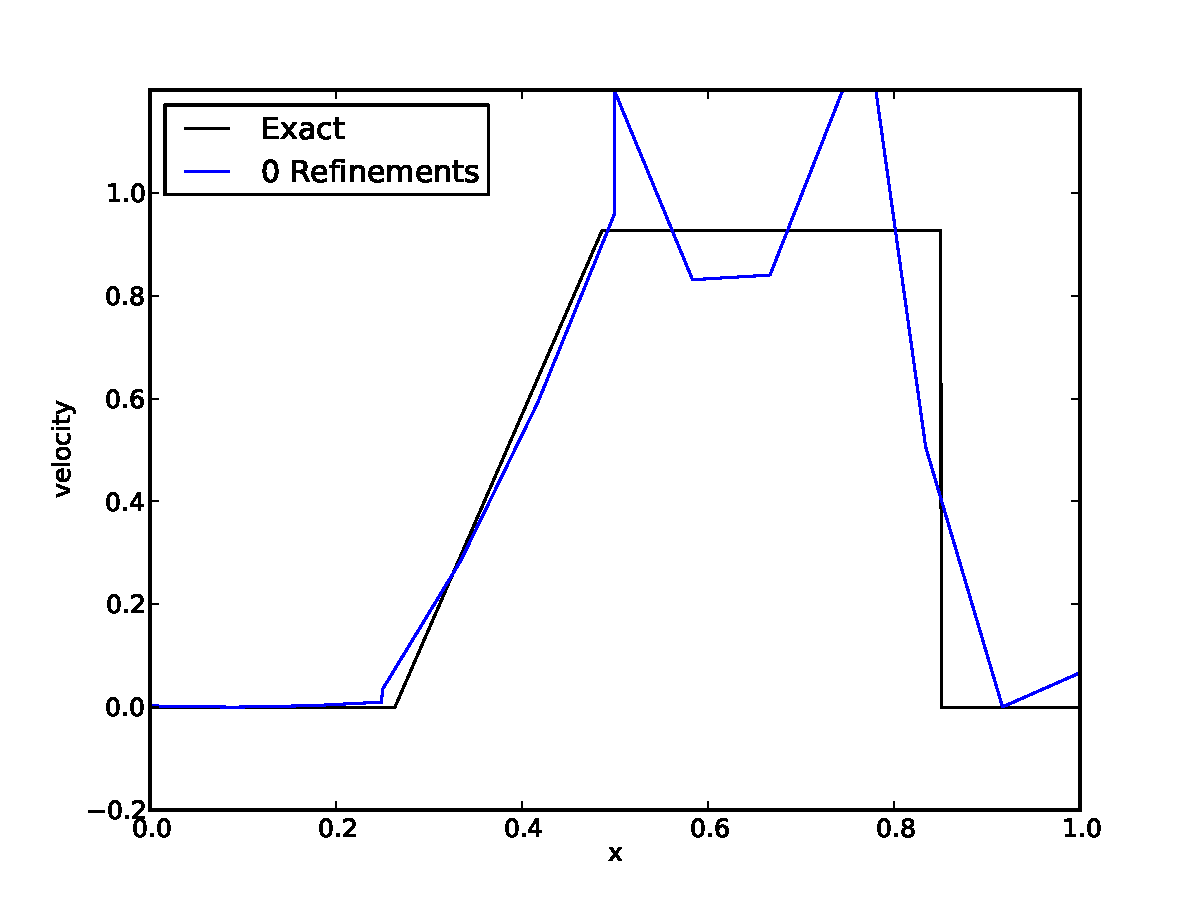
\includegraphics[width=\textwidth]{Dissertation/Sod/Robust-vel1.pdf}
\caption{Velocity}
\end{subfigure}
\begin{subfigure}[t]{0.45\textwidth}
\centering
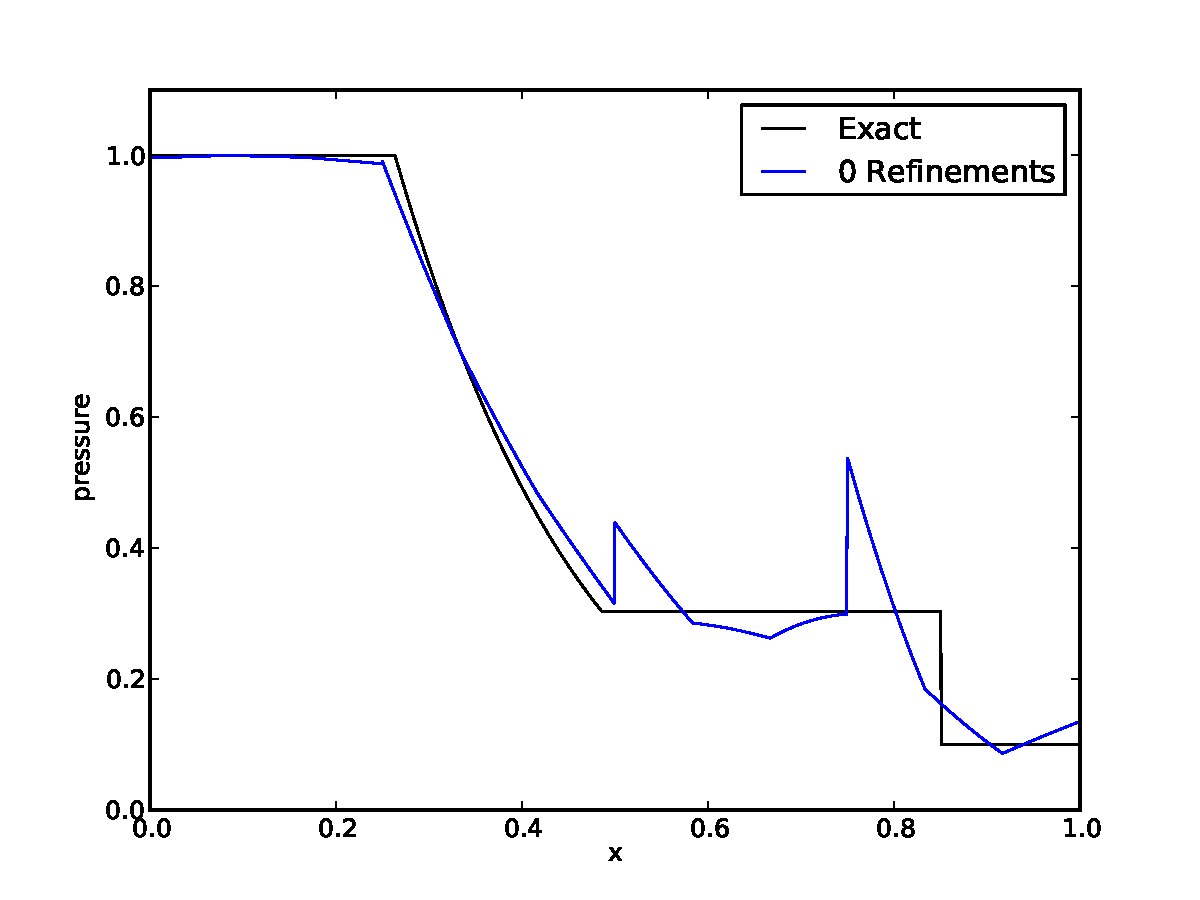
\includegraphics[width=\textwidth]{Dissertation/Sod/Robust-pres1.pdf}
\caption{Pressure}
\end{subfigure}
\begin{subfigure}[t]{0.9\textwidth}
\centering

\includegraphics[width=\textwidth]{Dissertation/Sod/Robust-mesh1.png}
\caption{Mesh}
\end{subfigure}
\caption{Sod solution with robust norm, initial mesh}
\label{fig:SodRobust0}
\end{figure}

\begin{figure}[ht]
\centering
\begin{subfigure}[t]{0.45\textwidth}
\centering
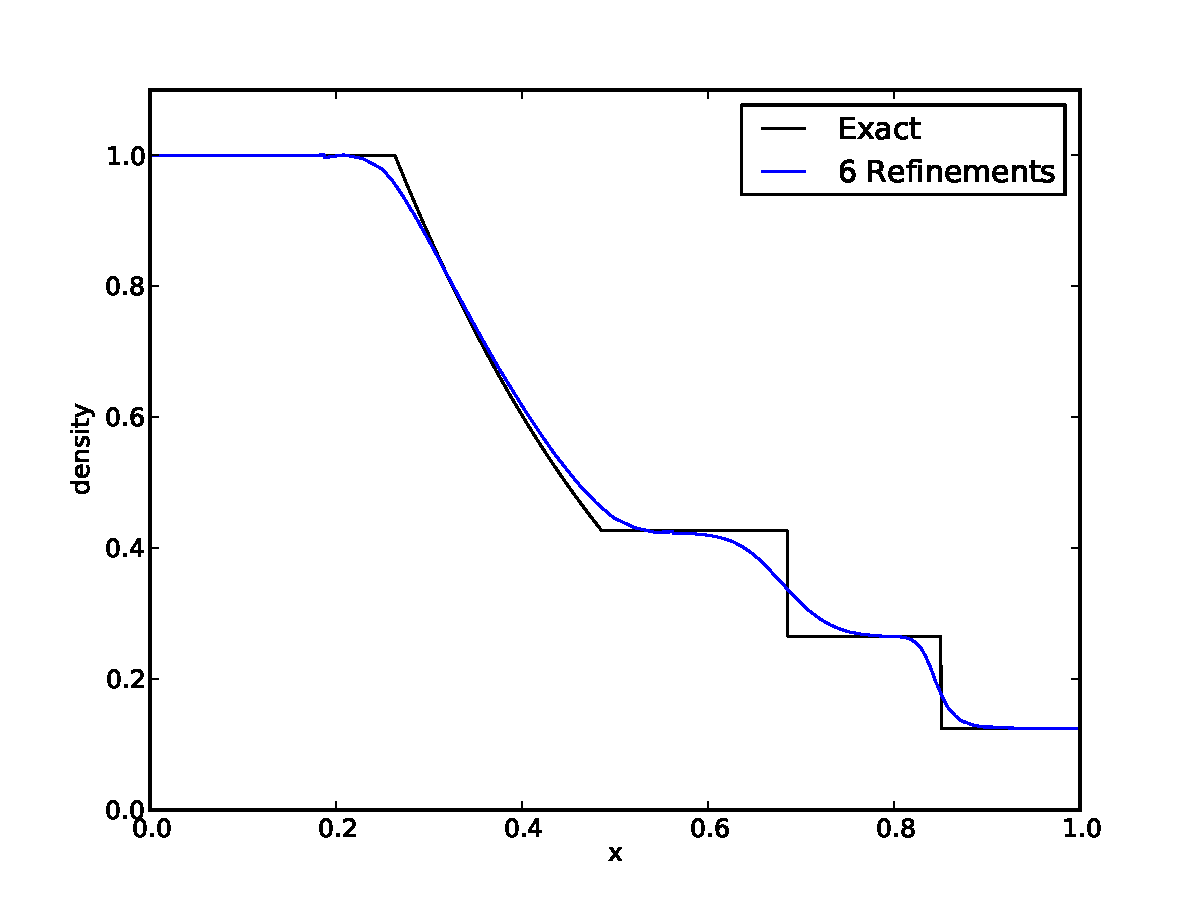
\includegraphics[width=\textwidth]{Dissertation/Sod/Robust-den7.pdf}
\caption{Density}
\end{subfigure}
\begin{subfigure}[t]{0.45\textwidth}
\centering
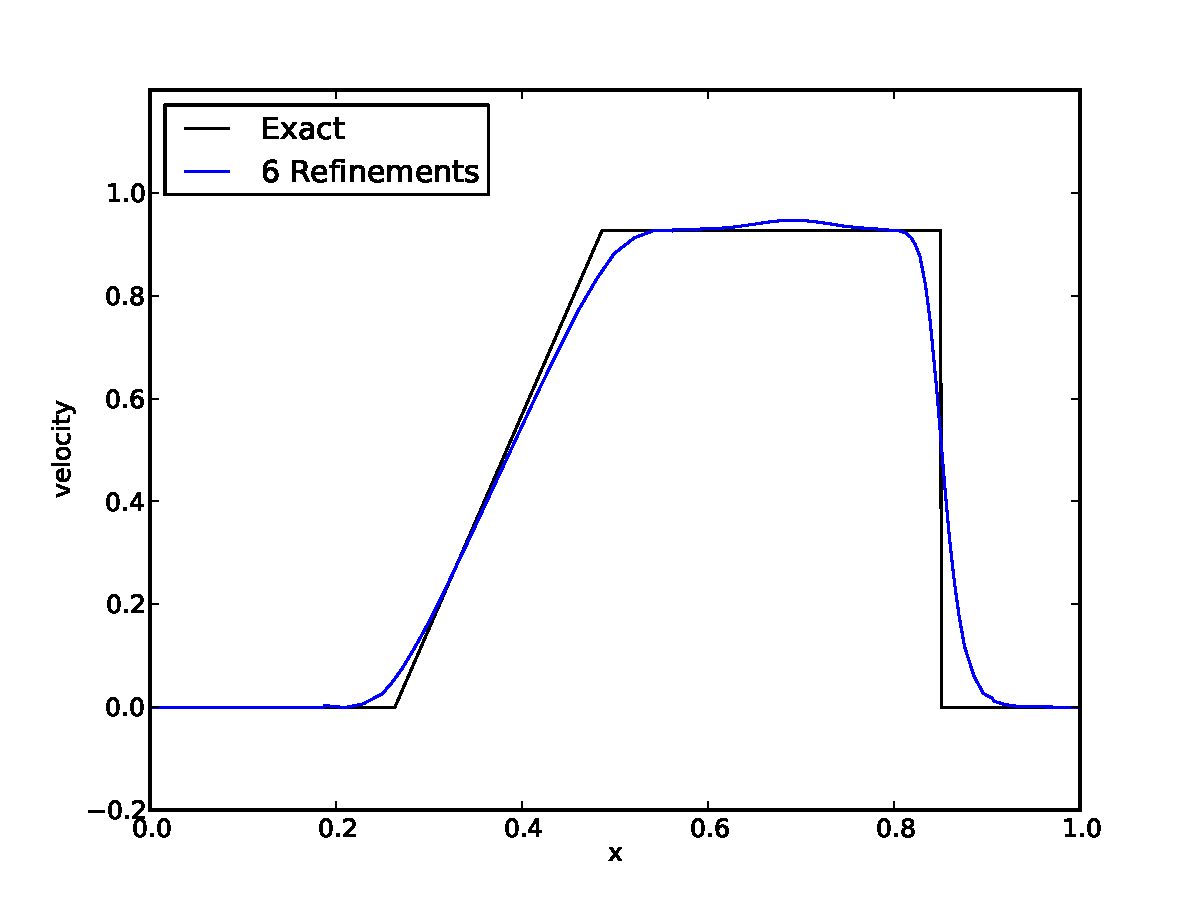
\includegraphics[width=\textwidth]{Dissertation/Sod/Robust-vel7.pdf}
\caption{Velocity}
\end{subfigure}
\begin{subfigure}[t]{0.45\textwidth}
\centering
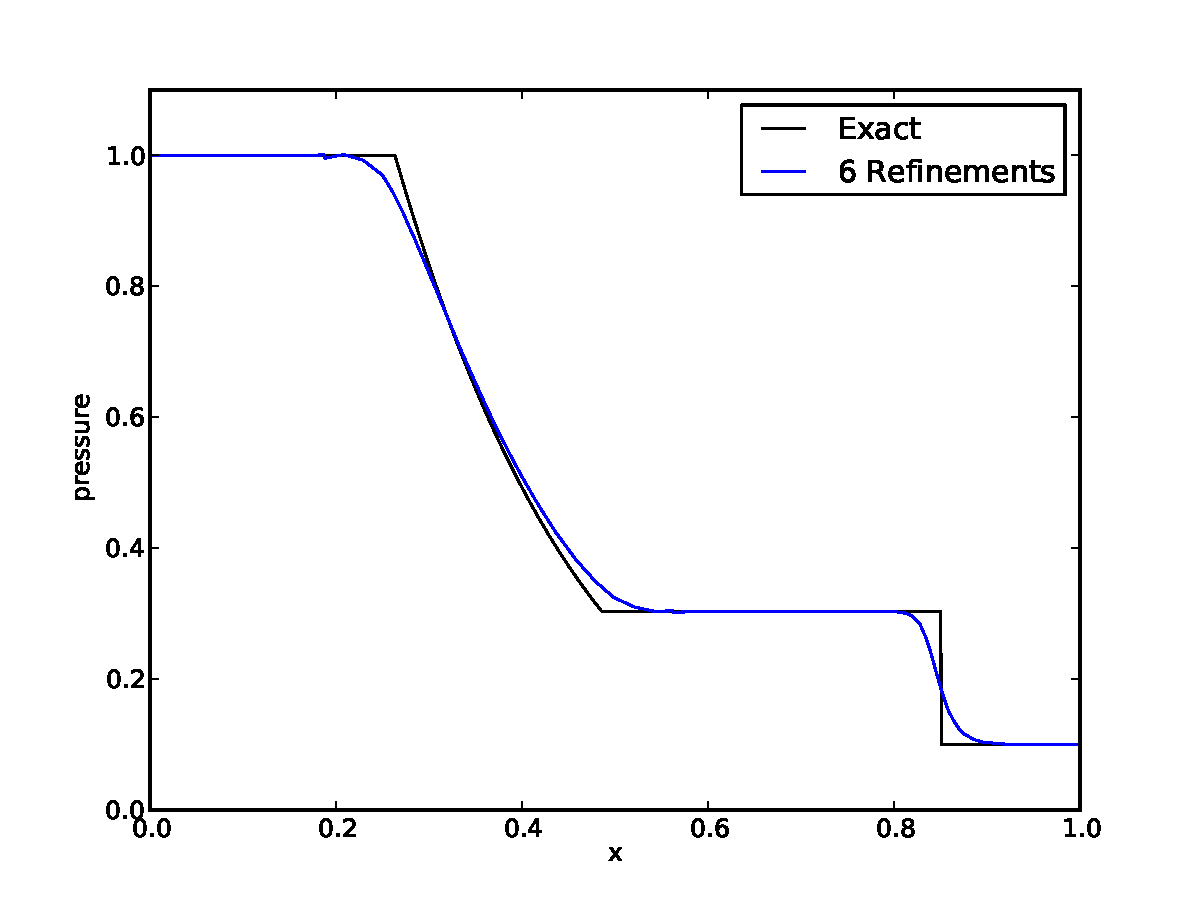
\includegraphics[width=\textwidth]{Dissertation/Sod/Robust-pres7.pdf}
\caption{Pressure}
\end{subfigure}
\begin{subfigure}[t]{0.9\textwidth}
\centering
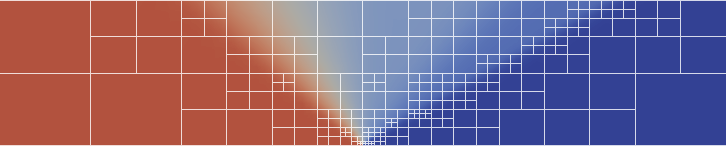
\includegraphics[width=\textwidth]{Dissertation/Sod/Robust-mesh7.png}
\caption{Mesh}
\end{subfigure}
\caption{Sod solution with robust norm, 6th refinement}
\label{fig:SodRobust6}
\end{figure}

\begin{figure}[ht]
\centering
\begin{subfigure}[t]{0.45\textwidth}
\centering
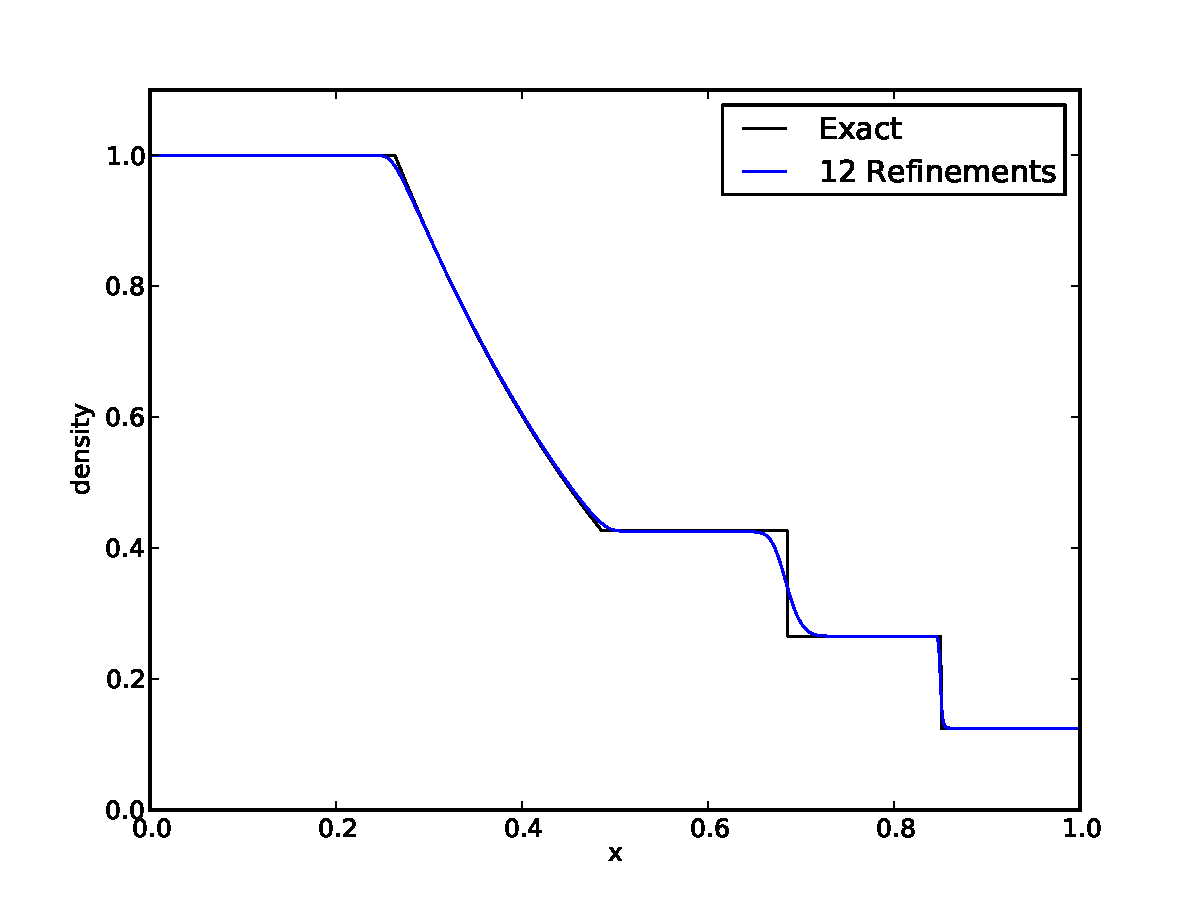
\includegraphics[width=\textwidth]{Dissertation/Sod/Robust-den13.pdf}
\caption{Density}
\end{subfigure}
\begin{subfigure}[t]{0.45\textwidth}
\centering
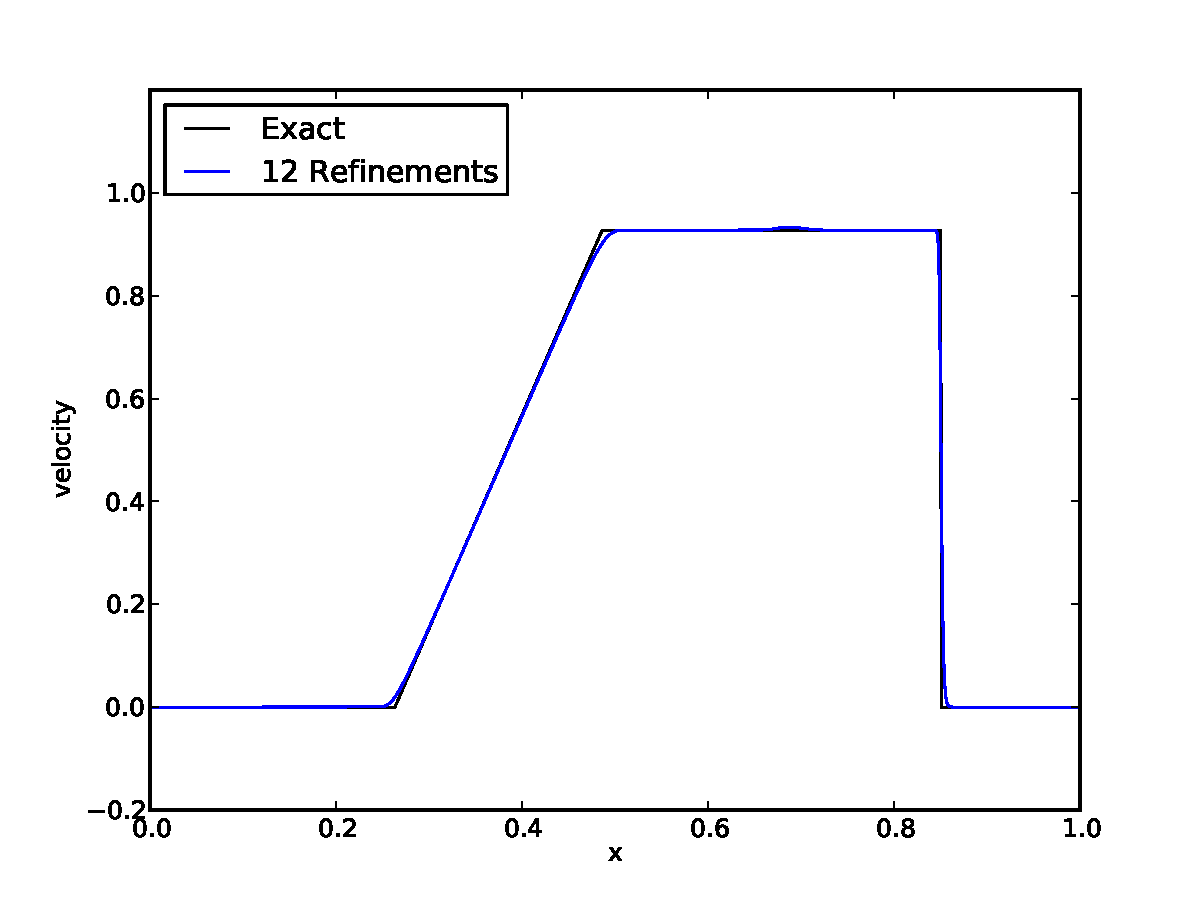
\includegraphics[width=\textwidth]{Dissertation/Sod/Robust-vel13.pdf}
\caption{Velocity}
\end{subfigure}
\begin{subfigure}[t]{0.45\textwidth}
\centering
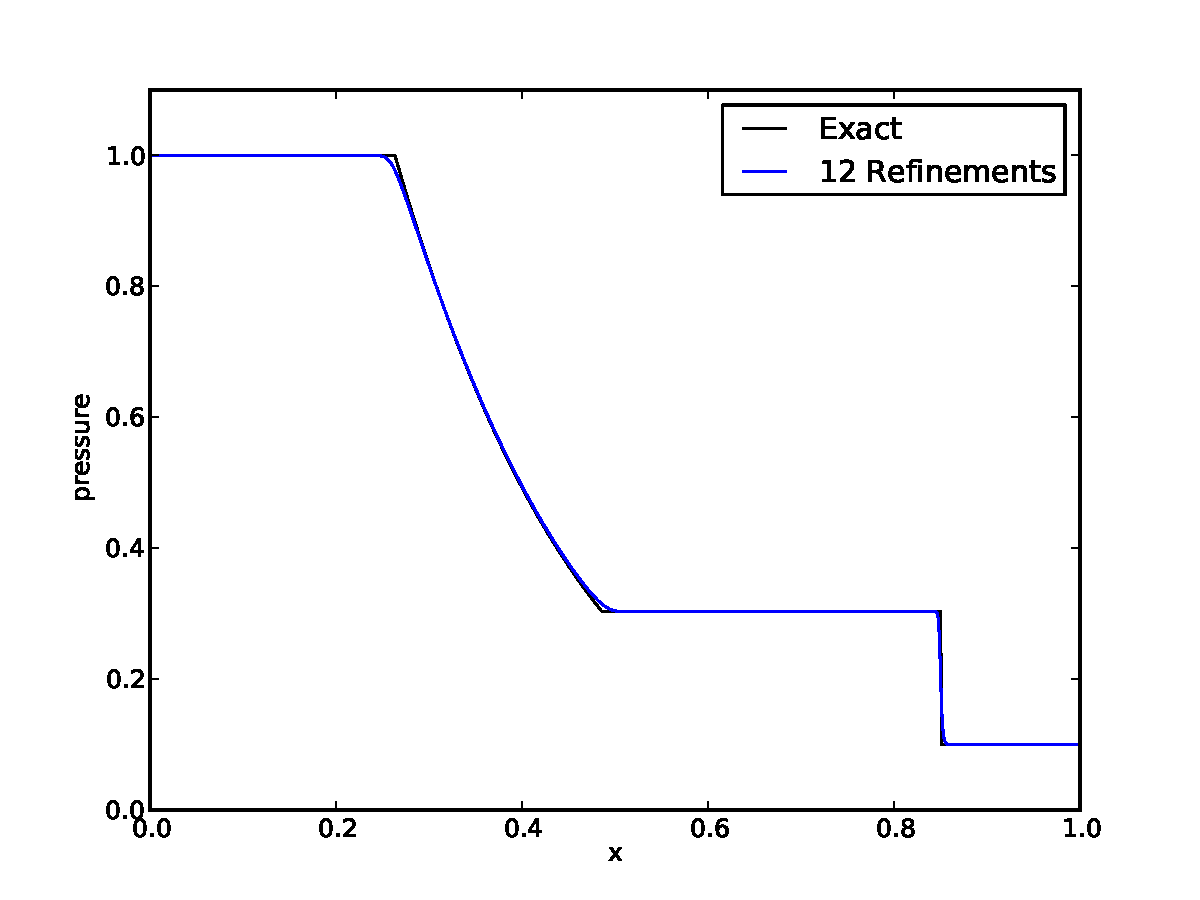
\includegraphics[width=\textwidth]{Dissertation/Sod/Robust-pres13.pdf}
\caption{Pressure}
\end{subfigure}
\begin{subfigure}[t]{0.9\textwidth}
\centering
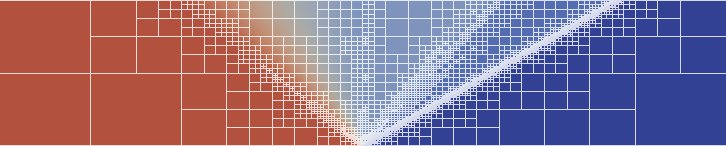
\includegraphics[width=\textwidth]{Dissertation/Sod/Robust-mesh13.png}
\caption{Mesh}
\end{subfigure}
\caption{Sod solution with robust norm, 12th refinement}
\label{fig:SodRobust12}
\end{figure}

\subsection{Noh Implosion}
% Re=1e3, p=1, delta_p=2, nlMaxIters=10, coarseRe=10

\begin{figure}[ht]
\centering
\begin{subfigure}[t]{0.32\textwidth}
\centering
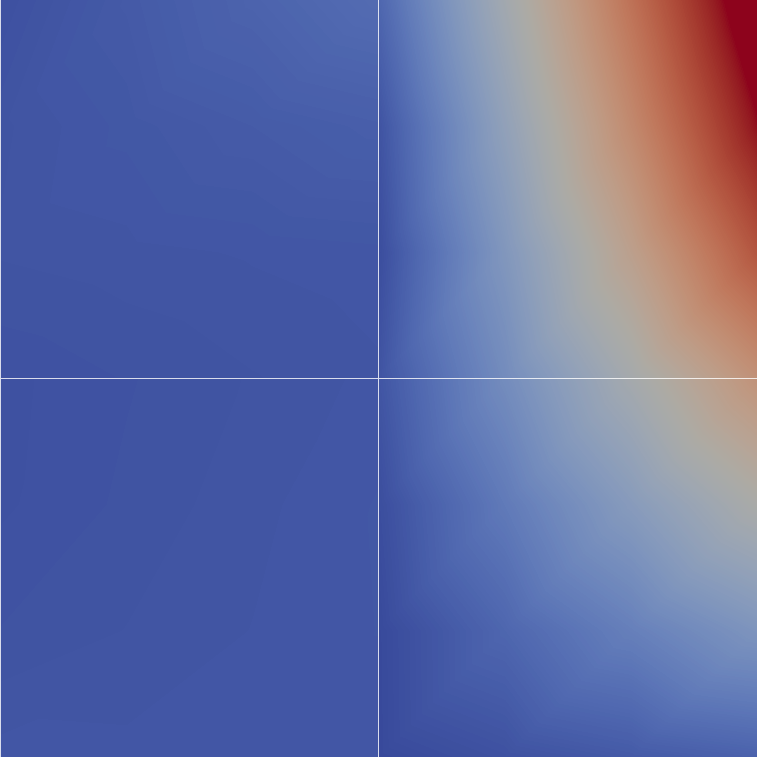
\includegraphics[width=\textwidth]{Dissertation/Noh/Robust-mesh0.png}
\caption{Initial Mesh}
\end{subfigure}
\begin{subfigure}[t]{0.32\textwidth}
\centering

\includegraphics[width=\textwidth]{Dissertation/Noh/Robust-mesh5.png}
\caption{After 5 refinements}
\end{subfigure}
\begin{subfigure}[t]{0.32\textwidth}
\centering
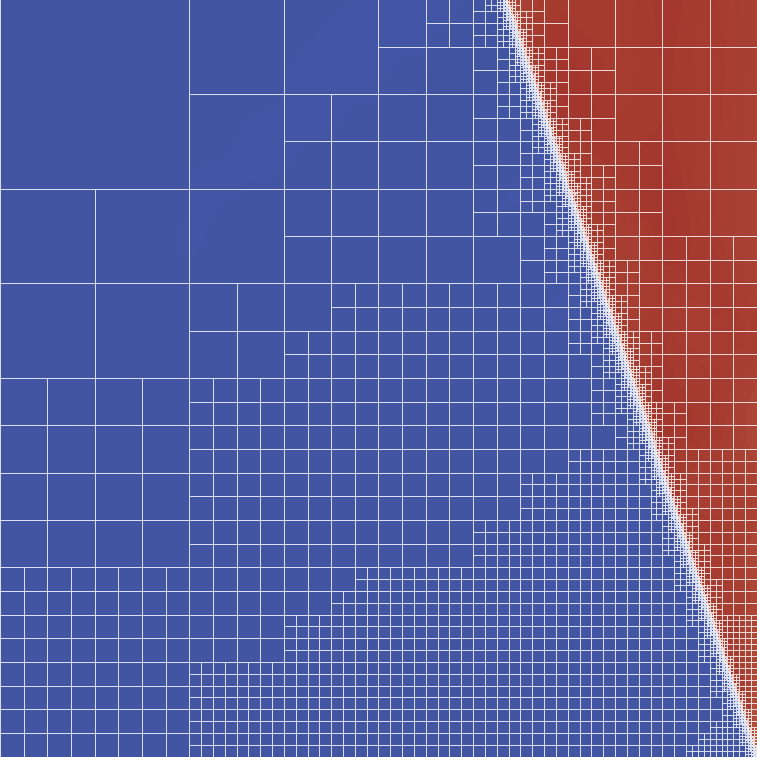
\includegraphics[width=\textwidth]{Dissertation/Noh/Robust-mesh10.png}
\caption{After 10 refinements}
\end{subfigure}
\begin{subfigure}[t]{0.9\textwidth}
\centering
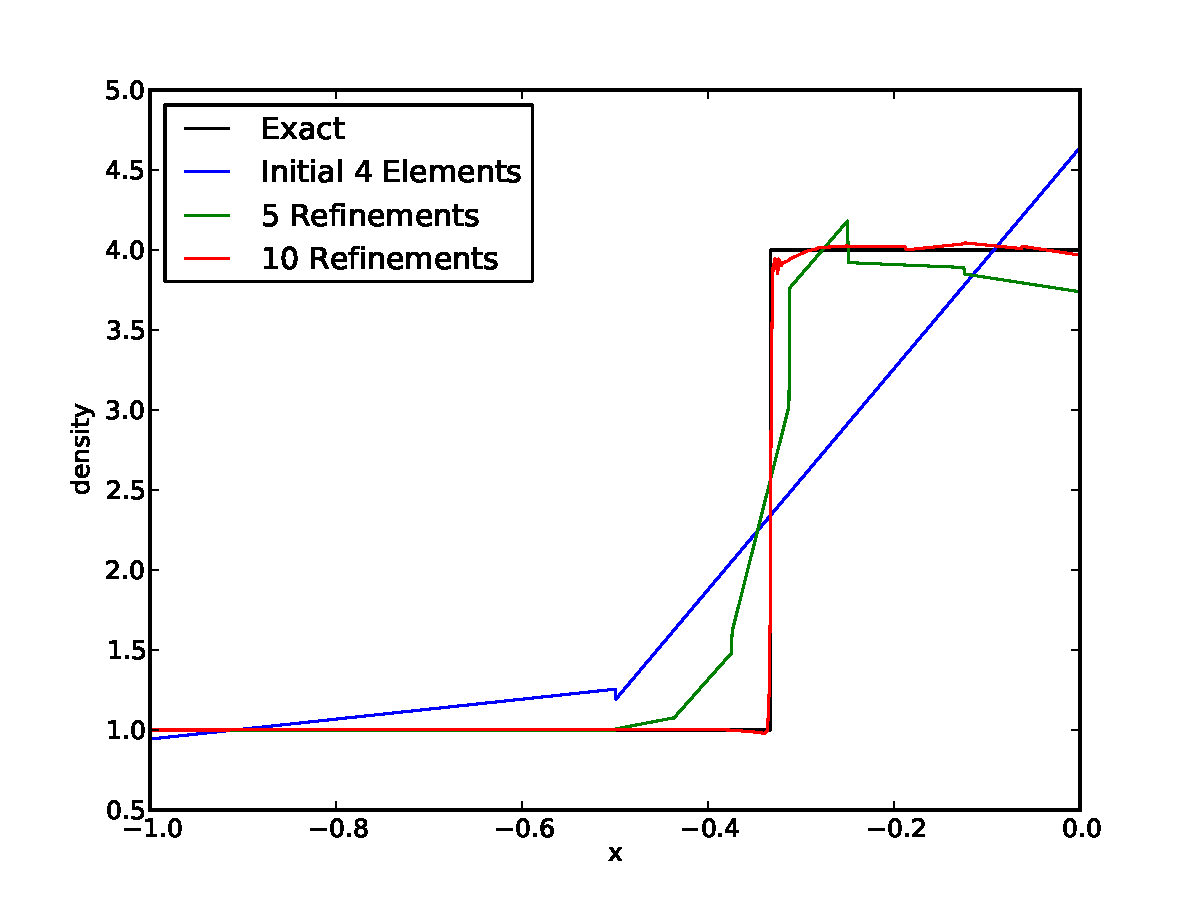
\includegraphics[width=\textwidth]{Dissertation/Noh/Robust-den.pdf}
\caption{Density at final time}
\end{subfigure}
\caption{Noh solution with robust norm}
\label{fig:NohRobustMesh}
\end{figure}

% \subsection{2D Space-Time Problems}

\end{document}
